\documentclass[twoside,a4wide,12pt]{article}\usepackage[]{graphicx}\usepackage[]{color}
%% maxwidth is the original width if it is less than linewidth
%% otherwise use linewidth (to make sure the graphics do not exceed the margin)
\makeatletter
\def\maxwidth{ %
  \ifdim\Gin@nat@width>\linewidth
    \linewidth
  \else
    \Gin@nat@width
  \fi
}
\makeatother

\definecolor{fgcolor}{rgb}{0.345, 0.345, 0.345}
\newcommand{\hlnum}[1]{\textcolor[rgb]{0.686,0.059,0.569}{#1}}%
\newcommand{\hlstr}[1]{\textcolor[rgb]{0.192,0.494,0.8}{#1}}%
\newcommand{\hlcom}[1]{\textcolor[rgb]{0.678,0.584,0.686}{\textit{#1}}}%
\newcommand{\hlopt}[1]{\textcolor[rgb]{0,0,0}{#1}}%
\newcommand{\hlstd}[1]{\textcolor[rgb]{0.345,0.345,0.345}{#1}}%
\newcommand{\hlkwa}[1]{\textcolor[rgb]{0.161,0.373,0.58}{\textbf{#1}}}%
\newcommand{\hlkwb}[1]{\textcolor[rgb]{0.69,0.353,0.396}{#1}}%
\newcommand{\hlkwc}[1]{\textcolor[rgb]{0.333,0.667,0.333}{#1}}%
\newcommand{\hlkwd}[1]{\textcolor[rgb]{0.737,0.353,0.396}{\textbf{#1}}}%

\usepackage{framed}
\makeatletter
\newenvironment{kframe}{%
 \def\at@end@of@kframe{}%
 \ifinner\ifhmode%
  \def\at@end@of@kframe{\end{minipage}}%
  \begin{minipage}{\columnwidth}%
 \fi\fi%
 \def\FrameCommand##1{\hskip\@totalleftmargin \hskip-\fboxsep
 \colorbox{shadecolor}{##1}\hskip-\fboxsep
     % There is no \\@totalrightmargin, so:
     \hskip-\linewidth \hskip-\@totalleftmargin \hskip\columnwidth}%
 \MakeFramed {\advance\hsize-\width
   \@totalleftmargin\z@ \linewidth\hsize
   \@setminipage}}%
 {\par\unskip\endMakeFramed%
 \at@end@of@kframe}
\makeatother

\definecolor{shadecolor}{rgb}{.97, .97, .97}
\definecolor{messagecolor}{rgb}{0, 0, 0}
\definecolor{warningcolor}{rgb}{1, 0, 1}
\definecolor{errorcolor}{rgb}{1, 0, 0}
\newenvironment{knitrout}{}{} % an empty environment to be redefined in TeX

\usepackage{alltt}
%\DefineVerbatimEnvironment{Sinput}{Verbatim} {xleftmargin=2em,frame=single}
%\DefineVerbatimEnvironment{Soutput}{Verbatim} {xleftmargin=2em,frame=single}
\usepackage[left=2.5cm,top=2cm,right=2cm,bottom=2.5cm,bindingoffset=0.5cm]{geometry}
\usepackage{amsmath} 
\usepackage[affil-it]{authblk}
\usepackage{hyperref}
\usepackage{fullpage}
\usepackage{pdflscape}
\usepackage[backend=bibtex,sorting=none,style=ieee]{biblatex}
\usepackage{setspace}
\bibliography{biblio}


\title{Proteochemometrics (PCM) with 'camb'\\
{\bf C}hemistry {\bf A}ware {\bf M}odel {\bf B}uilder\\
}

\author[1,3]{\rm Isidro Cortes-Ciriano\thanks{isidrolauscher@gmail.com}} 
\author[2,3]{\rm Daniel Murrell\thanks{dsmurrell@gmail.com}}
\affil[1]{Unite de Bioinformatique Structurale, Institut Pasteur and CNRS UMR 3825, Structural Biology and Chemistry Department, 25-28, rue Dr. Roux, 75 724 Paris, France.}
\affil[2]{Unilever Centre for Molecular Science Informatics, Department of Chemistry, University of Cambridge, Cambridge, United Kingdom.}
\affil[3]{Equal contributors}
\setlength{\parindent}{0pt}
\IfFileExists{upquote.sty}{\usepackage{upquote}}{}


\begin{document}

\maketitle
\onehalfspacing






\maketitle

In the following sections, we present a pipeline to generate a Proteochemometric (PCM) model for mammal cyclooxigenase (COX) inhibitors. 
Further details about this dataset are reserved for a future publication.
Similarly, the interested reader is referred to ref
\cite{review_pcm} and \cite{cortesReview} for futher details about PCM.

Firstly, the package needs to be loaded and the working directory specified:


\begin{knitrout}
\definecolor{shadecolor}{rgb}{0.969, 0.969, 0.969}\color{fgcolor}\begin{kframe}
\begin{alltt}
\hlkwd{library}\hlstd{(camb)}
\hlcom{# setwd('path_to_working_directory')}
\end{alltt}
\end{kframe}
\end{knitrout}


\section{Compounds}

\subsection{Reading and Preprocessing}
We proceed to read the compounds. Given that some smiles contain smarts patterns where the hash symbol is present, 
it is necessary to switch off the argument {\it comment.char} in order not to clip the smiles:
\begin{knitrout}
\definecolor{shadecolor}{rgb}{0.969, 0.969, 0.969}\color{fgcolor}\begin{kframe}
\begin{alltt}
\hlstd{smiles} \hlkwb{<-} \hlkwd{read.table}\hlstd{(}\hlstr{"smiles_COX.smi"}\hlstd{,} \hlkwc{header} \hlstd{=} \hlnum{FALSE}\hlstd{,}
    \hlkwc{comment.char} \hlstd{=} \hlkwd{c}\hlstd{(}\hlstr{""}\hlstd{))}
\end{alltt}
\end{kframe}
\end{knitrout}


The function {\it StandardiseMolecules} enables the depiction of molecular structures in the same (standardised) form.
The different arguments of this function allow control over the maximum number of (i) fluorines, (ii) chlorines,
(iii) bromines, and (iv) iodines the molecules contains in order to be retained for training.
Inorgnaic molecules (those containing atoms not in: \{H, C, N, O, P, S, F, Cl, Br, I\}) are removed if the argument "remove.inorganic" is set to "TRUE", which is the default value.
Additionally, upper and lower limits for the molecular mass can be set with the arguments "min.mass.limit" and "max.mass.limit".
The name of the file containing the chemical structures is input to the argument "structures.file".
\begin{knitrout}
\definecolor{shadecolor}{rgb}{0.969, 0.969, 0.969}\color{fgcolor}\begin{kframe}
\begin{alltt}
\hlkwd{StandardiseMolecules}\hlstd{(}\hlkwc{structures.file}\hlstd{=}\hlstr{"smiles_COX.smi"}\hlstd{,}
\hlkwc{standardised.file}\hlstd{=}\hlstr{"standardised.sdf"}\hlstd{,}
\hlkwc{removed.file}\hlstd{=}\hlstr{"removed.sdf"}\hlstd{,}
\hlkwc{output}\hlstd{=}\hlstr{"standardisation_COX_info.csv"}\hlstd{,}
\hlkwc{remove.inorganic}\hlstd{=}\hlnum{TRUE}\hlstd{,}
\hlkwc{fluorine.limit}\hlstd{=}\hlopt{-}\hlnum{1}\hlstd{,}
\hlkwc{chlorine.limit}\hlstd{=}\hlopt{-}\hlnum{1}\hlstd{,}
\hlkwc{bromine.limit}\hlstd{=}\hlopt{-}\hlnum{1}\hlstd{,}
\hlkwc{iodine.limit}\hlstd{=}\hlopt{-}\hlnum{1}\hlstd{,}
\hlkwc{min.mass.limit}\hlstd{=}\hlopt{-}\hlnum{1}\hlstd{,} \hlcom{#suggested value 20}
\hlkwc{max.mass.limit}\hlstd{=}\hlopt{-}\hlnum{1}\hlstd{)} \hlcom{#suggested value  900}
\end{alltt}
\end{kframe}
\end{knitrout}

The properties specified in the structure file of all molecules and an index, in the column "kept", indicating which molecules were deleted (0) and kept (1),
are written to the file indicated in the argument "properties.file", which is in CSV format.
In this case the file is \verb|"standardisation_COX_info.csv"|.
Molecules that Indigo manages to parse and that pass the filters are written to the file indicated in the argument "standardised.file".
By contrast, molecules that are discarded for training purposes are written to the file indicated in the argument "removed.file".

\begin{knitrout}
\definecolor{shadecolor}{rgb}{0.969, 0.969, 0.969}\color{fgcolor}\begin{kframe}
\begin{alltt}
\hlstd{standardised_info} \hlkwb{<-} \hlkwd{read.table}\hlstd{(}\hlstr{"standardisation_COX_info.csv"}\hlstd{,}
    \hlkwc{header} \hlstd{=} \hlnum{TRUE}\hlstd{,} \hlkwc{sep} \hlstd{=} \hlstr{"\textbackslash{}t"}\hlstd{)}
\end{alltt}
\end{kframe}
\end{knitrout}


Default values of the arguments of the function "StandardiseMolecules" are not stringent.
In the present case, all molecules are kept, thus all values in the columns "kept"
are equal to "1".

The values corresponding to an individual property in a ".sdf" file can be accessed with the function "GetPropertySDF".
Similarly, the function "GetPropertiesSDF" retrieves the information for all properties of a given ".sdf" file.
A data.frame with all properties is returned.
The number of molecules from which the information has to be retrieved can be indicated with the argument \verb|"number_processed"|.
The default value for this argument is \verb|"-1"|, which indicates that the properties will be extracted for all molecules in the input file.
\begin{knitrout}
\definecolor{shadecolor}{rgb}{0.969, 0.969, 0.969}\color{fgcolor}\begin{kframe}
\begin{alltt}
\hlkwd{ShowPropertiesSDF}\hlstd{(}\hlstr{"test.sdf"}\hlstd{)} \hlcom{# a mock .sdf file}
\hlkwd{GetPropertySDF}\hlstd{(}\hlstr{"test.sdf"}\hlstd{,}\hlkwc{property}\hlstd{=}\hlstr{"Name"}\hlstd{,}
               \hlkwc{number_processed}\hlstd{=}\hlnum{10}\hlstd{)}

\hlstd{all_properties} \hlkwb{<-} \hlkwd{GetPropertiesSDF}\hlstd{(}\hlstr{"test.sdf"}\hlstd{,}\hlkwc{number_processed}\hlstd{=}\hlnum{10}\hlstd{)}
\end{alltt}
\end{kframe}
\end{knitrout}


\subsection{PaDEL Descriptors}
One and two-dimensional PaDEL\cite{padel} descriptors and fingerprints can be calculated with the function "GeneratePadelDescriptors":
\begin{knitrout}
\definecolor{shadecolor}{rgb}{0.969, 0.969, 0.969}\color{fgcolor}\begin{kframe}
\begin{alltt}
descriptors_COX <- \hlkwd{GeneratePadelDescriptors}( +
  standardised.file=\hlstr{"smiles_COX.smi"},threads = 1)

descriptors <- \hlkwd{RemoveStandardisedPrefix}(descriptors)
\hlkwd{saveRDS}(descriptors, file=\hlstr{"Padel_COX.rds"})
descriptors <- \hlkwd{readRDS}(\hlstr{"Padel_COX.rds"})
\end{alltt}
\end{kframe}
\end{knitrout}


Sometimes, some descriptors are not calculated for all molecules, thus giving a "NA" or "Inf" as descriptor value.
Instead of removing that descriptor for all molecules, the missing descriptor values can be imputed from the corresponding descriptor values of the rest of molecules.
Descriptor values equal to "Inf" are converted to "NA".
For the imputation of missing descriptor values, the R package {\it impute} is required.
Depending on the R version, it can be accessed from either {\it CRAN} or {\it Bioconductor}.

\begin{knitrout}
\definecolor{shadecolor}{rgb}{0.969, 0.969, 0.969}\color{fgcolor}\begin{kframe}
\begin{alltt}
\hlstd{descriptors} \hlkwb{<-} \hlkwd{ReplaceInfinitesWithNA}\hlstd{(descriptors)}
\hlstd{descriptors} \hlkwb{<-} \hlkwd{ImputeFeatures}\hlstd{(descriptors)}
\end{alltt}
\end{kframe}
\end{knitrout}


\subsection{Circular Morgan Fingerprints}
The calculation of circular Morgan fingerprints requires the python library RDkit, given that the function "MorganFPs" calls a python script for the calculation of this type of fingerprints.
The python code is available in the "extdata" folder of the package or at:\\
https://github.com/isidroc/FingerprintCalculator.\\
For a detailed discussion about circular Morgan fingerprints, we refer
the interested reader to ref. \cite{morgan}.
When using integrated development environments (IDE) such as RStudio,
the environment variables might not be defined within the R session.
However, they can be redefined with the R function "Sys.setenv".
In any case, the function "MorganFPs" requires this information in the arguments "PythonPath", path to python in the system, and "RDkitPath", the path to the RDkit library. 
For instance, the information of the latter is contained in the environment variable \verb|$RDBASE| in Mac OS.

\begin{knitrout}
\definecolor{shadecolor}{rgb}{0.969, 0.969, 0.969}\color{fgcolor}\begin{kframe}
\begin{alltt}
\hlkwd{Sys.setenv}\hlstd{(}\hlkwc{RDBASE}\hlstd{=}\hlstr{"/usr/local/share/RDKit"}\hlstd{)}
\hlkwd{Sys.setenv}\hlstd{(}\hlkwc{PYTHONPATH}\hlstd{=}\hlstr{"/usr/local/lib/python2.7/site-packages"}\hlstd{)}

\hlstd{fps_COX_512} \hlkwb{<-} \hlkwd{MorganFPs}\hlstd{(}\hlkwc{bits}\hlstd{=}\hlnum{512}\hlstd{,}\hlkwc{radius}\hlstd{=}\hlnum{2}\hlstd{,}\hlkwc{type}\hlstd{=}\hlstr{'smi'}\hlstd{,}\hlkwc{mols}\hlstd{=}\hlstr{'smiles_COX.smi'}\hlstd{,}
                         \hlkwc{output}\hlstd{=}\hlstr{'COX'}\hlstd{,}\hlkwc{keep}\hlstd{=}\hlstr{'hashed_counts'}\hlstd{,}
                         \hlkwc{RDkitPath}\hlstd{=}\hlstr{'/usr/local/share/RDKit'}\hlstd{,}
                         \hlkwc{PythonPath}\hlstd{=}\hlstr{'/usr/local/lib/python2.7/site-packages'}\hlstd{,}
                         \hlkwc{verbose}\hlstd{=}\hlnum{TRUE}\hlstd{,} \hlkwc{images} \hlstd{=} \hlnum{FALSE}\hlstd{,} \hlkwc{unhashed} \hlstd{=} \hlnum{FALSE}\hlstd{,}
                         \hlkwc{extFileExtension} \hlstd{=} \hlnum{FALSE}\hlstd{,}
                         \hlkwc{extMols} \hlstd{=} \hlnum{FALSE}\hlstd{,} \hlkwc{unhashedExt} \hlstd{=} \hlnum{FALSE}\hlstd{,}
                         \hlkwc{logFile} \hlstd{=} \hlnum{FALSE}\hlstd{)}

\hlkwd{saveRDS}\hlstd{(fps_COX_512,}\hlkwc{file}\hlstd{=}\hlstr{"fps_COX_512.rds"}\hlstd{)}
\hlstd{fps_COX_512} \hlkwb{<-} \hlkwd{readRDS}\hlstd{(}\hlstr{"fps_COX_512.rds"}\hlstd{)}
\end{alltt}
\end{kframe}
\end{knitrout}


The function 'MorganFPs" enables the calculation of the following types of fingerprints:
\begin{itemize}

\item Hashed fingerprints in {\bf binary format} of a given number of bits (argument 'bits') considering substructures with a maximum radius, defined with the argument 'radius', for the molecules specified in the argument 'mols'. These fingerprints are dropped to the output file \verb|COX_hashed_binary.csv|, where output corresponds to the value of the argument 'output' ("COX" in the example presented above). 
In the calculation of hashed fingerprints, several substructures can be mapped to the same bit position.
Therefore, it might be important for the sake of interpretability to know which substructures are mapped to which bit in the fingerprint. This information is given in the file \verb|COX_features_per_bit_hashed_fp.csv|.
The first column of the file corresponds to the bit index, whereas the remaining columns correspond to substructure ids.
This file is created automatically every time the function is run.

\item Hashed fingerprints in {\bf counts format} of a given number of bits (argument 'bits') considering substructures with a maximum radius, defined with the argument 'radius', for the molecules specified in the argument 'mols'. These fingerprints are dropped to the output file \verb|COX_hashed_counts.csv|.

\item Unhashed fingerprints in {\bf binary format}. All substructures present in the input molecules (argument 'mols') are considered. Each position in the unhashed fingerprint corresponds to a given substructure. Thus, the resulting fingeprints are keyed. The smiles for each substructure and the number of atoms thereof is given in the output file \verb|COX_smiles_substructures.csv|. This file is created automatically every time the function is run. 
Unhashed fingerprints in {\bf binary format} are dropped to the output file \verb|COX_unhashed_binary.csv|.

\item Unhashed fingerprints in {\bf counts format}. All substructures present in the input molecules (argument 'mols') will be considered. Each position in the unhashed fingerprint corresponds to a given substructure. Thus, the resulting fingeprints are keyed. In contrast to binary format, where a given bit is set on if a substructure appears in a molecule irrespective of the number of times the substructure is present therein, the number of occurrences of each substructure is accounted. The smiles for each substructure and the number of atoms thereof is given in the output file \verb|COX_smiles_substructures.csv|,  whereas the fingerprints are dropped to the output file \verb|COX_unhashed_counts.csv|.

\item In those cases where a given predictive model has been built on unhashed fingeprints, the same fingerprints should be 
calcualted for new molecules for which predictions are to be made by that model. 
To this aim, the function "MorganFPs" enables the calculation of both hashed and unhashed fingerprints (in both binary and counts format) for the molecules present in a given file (hereinafter referred to as external file). The unhashed fingeprints will be calculated based on the pool of substructures present in the file indicated in the argument "mols".
To enable the calculation of fingerprints for the external file, the arguments "extMols" (name of the external file) and "extFileExtension" (file extension of the external file) need to be set. 
The hashed fingerprints will be dropped to the following files:\\
(i) binary format: \verb|{{\it output}}_hashed_binary_EXT.csv|, and (ii) counts format: 
\verb|{\it output}_hashed_counts_EXT.csv|.
If the user also wants the calculation of unhashed fingerprints for the molecules present in the external file, the argument "unhashedExt" needs to be set to TRUE. 
In this case the unhashed fingeprints will be dropped to the following files:\\
(i) binary format: \verb|{\it output}_unhashed_binary_EXT.csv|,\\
and (ii) counts format: \verb|{\it output}_unhashed_counts_EXT.csv|.

\end{itemize}

The indexes of the molecules that could not be handled during the calculation are dropped to the file \verb|incorrect_molecules_COX.csv|. Similarly, the indexes of the molecules from the external file that could not be processed are given in the file \verb|incorrect_molecules_EXT_COX.csv.|

In the following paragraph we describe in detail the arguments of the function "MorganFPs":
\begin{itemize}
\item {\bf bits:} Number of bits of the hashed fingerprints. The default value is 512.
\item {\bf radius:} Maximum radius of the substructures. A radius of 2 is equivalent to \verb|ECFP-4|, where 4 corresponds to the diameter. The default value is 2.
More information on ECFP fingerprints can be found here:\\
\verb|http://www.chemaxon.com/jchem/doc/user/ECFP.html|.
\item {\bf type:} File format containing the input molecules. The default value is ".smi".
\item {\bf mols:} File containing the input molecules.
\item {\bf output:} Label that will be appended to all ouput files (see below).
\item {\bf keep:} The fingeprints that will be kept after the calculation.
Apart from calculating different types of fingerprints, the function returns a data.frame with the type of fingerprints specified with this argument.  Possible types are: \verb|hashed_binary|,\verb|hashed_counts|, \verb|unhashed_binary|, \verb|unhashed_counts|, and if applicable,\\
\verb|hashed_binaryEXT|, \verb|hashed_countsEXT|, \verb|unhashed_binaryEXT|,\\
and \verb|unhashed_countsEXT|.
The default value is \verb|"hashed_binary"|.
\item {\bf images:} If TRUE, individual ".pdf" files containing (i) the image of each substructure in the context of a molecule presenting it, and (ii) each molecule correctly processed, are created.  Be aware that the number of substructures can be large depending on the number and diversity of the molecules present in the input file. Thus, allow for sufficient memory in those cases.
The default value is FALSE.
\item {\bf unhashed:} If TRUE, unhashed fingeprints, both in binary format and with counts, are calculated. The default value is FALSE.
\item {\bf verbose:} If TRUE, information about the progression of the calculation is printed. The default value is FALSE.
\item {\bf RDkitPath:} The path to the folder containing the RDkit library in your computer. On mac, the environment variable \verb|$RDBASE| contains this information. The default value is "/usr/local/share/RDKit".
\item {\bf PythonPath:} Path to python (\verb|$PYTHONPATH|).\\
The default value is "/usr/local/lib/python2.7/site-packages".
\item {\bf extFileExtension:} If not FALSE, file extension for the external file containing the molecules for which unhashed fingeprints are to be calculated with respect to the pool of substructures in the molecules present in the file specified in "mols". The default value is FALSE.
\item {\bf extMols:} If not FALSE, external file containing the molecules for which unhashed fingeprints are to be calculated with respect to the pool of
substructures in the molecules present in the file specified in "mols". The default value is FALSE.
\item {\bf unhashedExt:} If TRUE, unhashed fingerprints are calcualted for the molecules specified in "extMols". The default value is FALSE.
\item {\bf logFile:} If not FALSE, file where the log messages will be dropped. The default value is FALSE.
\end{itemize}


\section{Targets}

In the following section the tools provided by {\it camb} to calculate amino acid and whole protein descriptors will be presented.

\subsection{Reading and Preprocessing the Amino Acid Descriptors}
In the current example, the amino acids implicated in ligand binding were extracted from the binding site of the ovine cyclooxygenase 1 (PDB ID: 3KK6). The corresponding amino acids for the rest of mammal cyclooxygenases were defined by sequence alignment.
The amino acids corresponding to the target part of each compound-target combination in the dataset are given in the file \verb|"AAs_COX.csv"|. Thus, the number of rows of this file corresponds to the number of datapoints in the dataset.
We proceed to read the amino acids from the ".csv" file:
\begin{knitrout}
\definecolor{shadecolor}{rgb}{0.969, 0.969, 0.969}\color{fgcolor}\begin{kframe}
\begin{alltt}
\hlstd{amino_acid_IDs} \hlkwb{<-} \hlkwd{read.table}\hlstd{(}\hlstr{"AAs_COX.csv"}\hlstd{,} \hlkwc{sep} \hlstd{=} \hlstr{","}\hlstd{,}
    \hlkwc{header} \hlstd{=} \hlnum{TRUE}\hlstd{,} \hlkwc{colClasses} \hlstd{=} \hlkwd{c}\hlstd{(}\hlstr{"character"}\hlstd{),} \hlkwc{row.names} \hlstd{=} \hlnum{1}\hlstd{)}
\hlstd{amino_acid_IDs} \hlkwb{<-} \hlstd{amino_acid_IDs[,} \hlnum{2}\hlopt{:}\hlkwd{ncol}\hlstd{(amino_acid_IDs)]}
\end{alltt}
\end{kframe}
\end{knitrout}

Subsequently, 5 \verb|Z-scales| will be calculated, which will serve to describe the target space in the PCM models.
The descriptors will be saved to a ".rds" file.
\begin{knitrout}
\definecolor{shadecolor}{rgb}{0.969, 0.969, 0.969}\color{fgcolor}\begin{kframe}
\begin{alltt}
\hlstd{amino_acid_IDs_zscales} \hlkwb{<-} \hlkwd{AADescs}\hlstd{(}\hlkwc{Data} \hlstd{= amino_acid_IDs,}
    \hlkwc{type} \hlstd{=} \hlstr{"Z5"}\hlstd{)}
\hlkwd{saveRDS}\hlstd{(amino_acid_IDs_zscales,} \hlkwc{file} \hlstd{=} \hlstr{"Z5_COX.rds"}\hlstd{)}
\hlstd{amino_acid_IDs_zscales} \hlkwb{<-} \hlkwd{readRDS}\hlstd{(}\hlstr{"Z5_COX.rds"}\hlstd{)}
\end{alltt}
\end{kframe}
\end{knitrout}




The function \verb|"AA_descs"| permits the calculation of the following types of amino acid descriptors (futher details about these amino acid descriptors can be found in refs \cite{AAs1} and \cite{AAs2}):
\begin{itemize}
\item ProtFP8
\item T-Scales
\item VHSE
\item ST-Scales
\item BLOSUM
\item FASGAI
\item MSWHIM
\item 5 Z-Scales
\item 3 Z-Scales
\end{itemize}
This function outputs a data.frame which columns are indexed by the descriptors, and rows by the datapoints. Thus, the number of rows in the original data.frame or matrix, and the number of rows of the ouput data.frame are equal. 
If several descriptor types are chosen, by providing a vector of strings to the argument "type", descriptors are concatenated for the ease of further modeling. 
For instance: 
\begin{knitrout}
\definecolor{shadecolor}{rgb}{0.969, 0.969, 0.969}\color{fgcolor}\begin{kframe}
\begin{alltt}
\hlkwd{AA_descs}\hlstd{(}\hlkwc{Data} \hlstd{=} \hlkwd{c}\hlstd{(}\hlstr{"Ala"}\hlstd{),} \hlkwc{type} \hlstd{=} \hlkwd{c}\hlstd{(}\hlstr{"Z5"}\hlstd{,} \hlstr{"BLOSUM"}\hlstd{))}
\end{alltt}


{\ttfamily\noindent\bfseries\color{errorcolor}{\#\# Error: could not find function "{}AA\_descs"{}}}\end{kframe}
\end{knitrout}

Column names indicate the amino acid position in the original input data, and the type of descriptor.
\\
Whole sequence descriptors can be computed with the function "SeqDescs". 
The function takes as argument either a UniProt identifier, or either a matrix or dataframe with the protein sequences.
If a UniProt identifier is provided, the function gets firstly the sequence and then calculates the descriptors on the sequence.

\begin{knitrout}
\definecolor{shadecolor}{rgb}{0.969, 0.969, 0.969}\color{fgcolor}\begin{kframe}
\begin{alltt}
\hlstd{Seq_descriptors_P00374} \hlkwb{<-} \hlkwd{SeqDescs}\hlstd{(}\hlstr{"P00374"}\hlstd{,} \hlkwc{UniProtID} \hlstd{=} \hlnum{TRUE}\hlstd{,}
    \hlkwc{type} \hlstd{=} \hlkwd{c}\hlstd{(}\hlstr{"AAC"}\hlstd{,} \hlstr{"DC"}\hlstd{))}
\end{alltt}
\end{kframe}
\end{knitrout}

The available types of whole sequence descriptors are:\cite{protr}
\begin{itemize}
\item Amino Acid Composition ("AAC")
\item Dipeptide Composition ("DC")
\item Tripeptide Composition ("TC")
\item Normalized Moreau-Broto Autocorrelation ("MoreauBroto")
\item Moran Autocorrelation ("Moran")
\item Geary Autocorrelation ("Geary")
\item  CTD (Composition/Transition/Distribution) ("CTD")
\item Conjoint Traid ("CTriad")
\item Sequence Order Coupling Number ("SOCN")
\item Quasi-sequence Order Descriptors ("QSO")
\item Pseudo Amino Acid Composition ("PACC")
\item Amphiphilic Pseudo Amino Acid Composition ("APAAC")
\end{itemize}

\subsection{Reading the Dataset Information}
In the following subsection, 
the file containing the information about the dataset, namely: target names, bioctivities, etc.., wil be read.
Note that when reading molecules in smiles format from a ".csv" file into an R dataframe, the smiles are clipped after a hash ("\#") symbol.
A good practice is thus to also keep the smiles alone in a separate \{.smi,.smiles\} file.

\begin{knitrout}
\definecolor{shadecolor}{rgb}{0.969, 0.969, 0.969}\color{fgcolor}\begin{kframe}
\begin{alltt}
\hlstd{dataset} \hlkwb{<-} \hlkwd{readRDS}\hlstd{(}\hlstr{"COX_dataset_info.rds"}\hlstd{)}
\hlstd{bioactivity} \hlkwb{<-} \hlstd{dataset}\hlopt{$}\hlstd{standard_value}
\end{alltt}
\end{kframe}
\end{knitrout}

The bioactivity is in nM. We convert it to pIC50. To do that, we multiply by \verb|10^-9| to convert the bioactivity units to M.
Subsequently, the negative logarithm to base 10 is calculated:
\begin{knitrout}
\definecolor{shadecolor}{rgb}{0.969, 0.969, 0.969}\color{fgcolor}\begin{kframe}
\begin{alltt}
\hlstd{bioactivity} \hlkwb{<-} \hlstd{bioactivity} \hlopt{*} \hlnum{10}\hlopt{^-}\hlnum{9}
\hlstd{bioactivity} \hlkwb{<-} \hlopt{-}\hlkwd{log}\hlstd{(bioactivity,} \hlkwc{base} \hlstd{=} \hlnum{10}\hlstd{)}
\end{alltt}
\end{kframe}
\end{knitrout}


\section{Dataset Visualization}
Compounds can be depicted with the function "PlotMolecules".
This function returns a list of four plots. Additionally, plots can also be written into a ".pdf" file if the argument "pdf.file" is not NULL. The argument "IDs" corresponds to the index of the molecules in the input file which are to be depicted.
The name of the molecule in the input file will be used as the title of the image if the argument "useNameAsTitle" is set to TRUE.




\begin{knitrout}
\definecolor{shadecolor}{rgb}{0.969, 0.969, 0.969}\color{fgcolor}\begin{kframe}
\begin{alltt}
\hlstd{plot_molecules} \hlkwb{<-} \hlkwd{PlotMolecules}\hlstd{(}\hlstr{"standardised.sdf"}\hlstd{,}
    \hlkwc{IDs} \hlstd{=} \hlkwd{c}\hlstd{(}\hlnum{1}\hlstd{,} \hlnum{2}\hlstd{,} \hlnum{3}\hlstd{,} \hlnum{4}\hlstd{),} \hlkwc{pdf.file} \hlstd{=} \hlkwa{NULL}\hlstd{,} \hlkwc{useNameAsTitle} \hlstd{=} \hlnum{TRUE}\hlstd{,}
    \hlkwc{PDFMain} \hlstd{=} \hlkwa{NULL}\hlstd{)}
\end{alltt}


{\ttfamily\noindent\bfseries\color{errorcolor}{\#\# Error: could not find function "{}DrawMoleculeInSDF"{}}}\begin{alltt}
\hlkwd{print}\hlstd{(plot_molecules[[}\hlnum{1}\hlstd{]])}
\end{alltt}


{\ttfamily\noindent\bfseries\color{errorcolor}{\#\# Error: object 'plot\_molecules' not found}}\end{kframe}
\end{knitrout}


The distribution of the response variable can be explored with the function "DensityResponse" in the following way: 
\begin{knitrout}
\definecolor{shadecolor}{rgb}{0.969, 0.969, 0.969}\color{fgcolor}\begin{kframe}
\begin{alltt}
\hlstd{dens_resp} \hlkwb{<-} \hlkwd{DensityResponse}\hlstd{(bioactivity,} \hlkwc{xlab} \hlstd{=} \hlstr{"pIC50"}\hlstd{,}
    \hlkwc{main} \hlstd{=} \hlstr{""}\hlstd{,} \hlkwc{ylab} \hlstd{=} \hlstr{"Densitiy"}\hlstd{,} \hlkwc{TitleSize} \hlstd{=} \hlnum{30}\hlstd{,} \hlkwc{XAxisSize} \hlstd{=} \hlnum{22}\hlstd{,}
    \hlkwc{YAxisSize} \hlstd{=} \hlnum{22}\hlstd{,} \hlkwc{TitleAxesSize} \hlstd{=} \hlnum{24}\hlstd{,} \hlkwc{AngleLab} \hlstd{=} \hlnum{0}\hlstd{,}
    \hlkwc{lmar} \hlstd{=} \hlnum{0}\hlstd{,} \hlkwc{rmar} \hlstd{=} \hlnum{0}\hlstd{,} \hlkwc{bmar} \hlstd{=} \hlnum{0}\hlstd{,} \hlkwc{tmar} \hlstd{=} \hlnum{0}\hlstd{,} \hlkwc{binwidth} \hlstd{=} \hlnum{0.3}\hlstd{)}
\end{alltt}
\end{kframe}
\end{knitrout}

Given that the output of the function "DensityResponse" is a ggplot2 object, additional layers can be added to further customize the image.
A common analysis in bio- and chemoinformatics is to run a Pricipal Component Analysis (PCA) of either compound or target descriptors. 
The function "PCAProt" enables the calculation of the Principal Components (PCs) for a given set of descriptors.
The function takes as arguments the descriptors and, optionally, the names of the rows, {\it i.e.} datapoints.
Further arguments of the function {\it prcomp} from the package {\it stats}, use to run the PCA analysis, can be additionally set.
The function returns a list with following elements :
\begin{itemize}
\item Data : a dataframe containing the two first PCs and the row names if provided. 
Rows are indexed as in the input data corresponds to a list.
\item \verb|PCs_All| : a dataframe containing all PCs.
\item Std : a vector containing the standard deviation of all PCs.
\item Info : information about the PCA analysis, such as the proportion of variance explained by each PC.
It is always advisable to verify that the two or three first PCs explain a large proportion of the variance in the data,
if conclusions are to be extracted from this type of analysis.
\end{itemize}
The function "PCAPlot" provides an easy way to plot the first two PC. 
As all the plotting function provided with {\it camb}, it is based on 
{\it ggplot2}, which allows further customization by the user.
Below is an example of how to use these two function to do a PCA analysis of the target space, 
which in this case is quantified by the amino acid descriptors of the amino acids present in the binding site
of mammal cyclooxygenases.
\begin{knitrout}
\definecolor{shadecolor}{rgb}{0.969, 0.969, 0.969}\color{fgcolor}\begin{kframe}
\begin{alltt}
\hlstd{target_PCA} \hlkwb{<-} \hlkwd{PCA}\hlstd{(}\hlkwc{Data}\hlstd{=amino_acid_IDs_zscales,}
                  \hlkwc{RowNames}\hlstd{=dataset}\hlopt{$}\hlstd{accession,}
                  \hlkwc{cor}\hlstd{=}\hlnum{TRUE}\hlstd{,}\hlkwc{scale} \hlstd{=} \hlnum{TRUE}\hlstd{,}
                  \hlkwc{center} \hlstd{=} \hlnum{TRUE}\hlstd{)}

\hlstd{plot_PCA_COX} \hlkwb{<-} \hlkwd{PCAPlot}\hlstd{(target_PCA}\hlopt{$}\hlstd{Data,}\hlkwc{PointSize}\hlstd{=}\hlnum{10}\hlstd{,}\hlkwc{main}\hlstd{=}\hlstr{""}\hlstd{,}
                  \hlkwc{TitleSize}\hlstd{=}\hlnum{30}\hlstd{,}\hlkwc{XAxisSize}\hlstd{=}\hlnum{20}\hlstd{,}\hlkwc{YAxisSize}\hlstd{=}\hlnum{20}\hlstd{,}
                  \hlkwc{TitleAxesSize}\hlstd{=}\hlnum{28}\hlstd{,}\hlkwc{LegendPosition}\hlstd{=}\hlstr{"bottom"}\hlstd{,}
                  \hlkwc{RowLegend}\hlstd{=}\hlnum{3}\hlstd{,}\hlkwc{ColLegend}\hlstd{=}\hlnum{5}\hlstd{,}\hlkwc{LegendTitleSize}\hlstd{=}\hlnum{15}\hlstd{,}
                  \hlkwc{LegendTextSize}\hlstd{=}\hlnum{15}\hlstd{)}
\end{alltt}
\end{kframe}
\end{knitrout}


Similarly, the chemical space can be explored by calculating pairwise compound similarities based upon compound descriptors. 
In this case, we use the Jaccard metric to calculate the distance between compounds.
See the documentation of the {\it vegan} package for further information about other dissimilarity indices available.
The function "PairwiseDist" is based on the function "vegdist" from the package {\it vegan}.
Further arguments specified in the function "PairwiseDist" will be passed to the function "vegdist". 
For illustration, the argument "na.rm" will be given below to the "PairwiseDist" function, which will be in turn
passed to the function "vegdist".
\begin{knitrout}
\definecolor{shadecolor}{rgb}{0.969, 0.969, 0.969}\color{fgcolor}\begin{kframe}
\begin{alltt}
\hlstd{pw_dist_comp_fps} \hlkwb{<-} \hlkwd{PairwiseDist}\hlstd{(fps_COX_512,} \hlkwc{method} \hlstd{=} \hlstr{"jaccard"}\hlstd{,}
    \hlkwc{na.rm} \hlstd{=} \hlnum{TRUE}\hlstd{)}
\hlkwd{saveRDS}\hlstd{(pw_dist_comp_fps,} \hlkwc{file} \hlstd{=} \hlstr{"pairwise_dist_COX.rds"}\hlstd{)}
\end{alltt}
\end{kframe}
\end{knitrout}

The dissimilarity distribution can be depicted with the function "PairwiseDistPlot": 
\begin{knitrout}
\definecolor{shadecolor}{rgb}{0.969, 0.969, 0.969}\color{fgcolor}\begin{kframe}
\begin{alltt}
\hlstd{pw_dist_comp_fps} \hlkwb{<-} \hlkwd{readRDS}\hlstd{(}\hlstr{"pairwise_dist_COX.rds"}\hlstd{)}
\hlstd{plot_pwd} \hlkwb{<-} \hlkwd{PairwiseDistPlot}\hlstd{(pw_dist_comp_fps,} \hlkwc{xlab} \hlstd{=} \hlstr{"Jaccard Index"}\hlstd{,}
    \hlkwc{ylab} \hlstd{=} \hlstr{"Density"}\hlstd{,} \hlkwc{TitleSize} \hlstd{=} \hlnum{26}\hlstd{,} \hlkwc{XAxisSize} \hlstd{=} \hlnum{20}\hlstd{,}
    \hlkwc{YAxisSize} \hlstd{=} \hlnum{20}\hlstd{,} \hlkwc{TitleAxesSize} \hlstd{=} \hlnum{24}\hlstd{,} \hlkwc{lmar} \hlstd{=} \hlnum{0}\hlstd{,} \hlkwc{rmar} \hlstd{=} \hlnum{0}\hlstd{,}
    \hlkwc{bmar} \hlstd{=} \hlnum{0}\hlstd{,} \hlkwc{tmar} \hlstd{=} \hlnum{0}\hlstd{,} \hlkwc{AngleLab} \hlstd{=} \hlnum{0}\hlstd{)}
\end{alltt}
\end{kframe}
\end{knitrout}


\begin{knitrout}
\definecolor{shadecolor}{rgb}{0.969, 0.969, 0.969}\color{fgcolor}\begin{kframe}
\begin{alltt}
\hlkwd{grid.arrange}\hlstd{(dens_resp, plot_pwd,} \hlkwc{nrow} \hlstd{=} \hlnum{2}\hlstd{)}
\end{alltt}
\end{kframe}\begin{figure}[]


{\centering 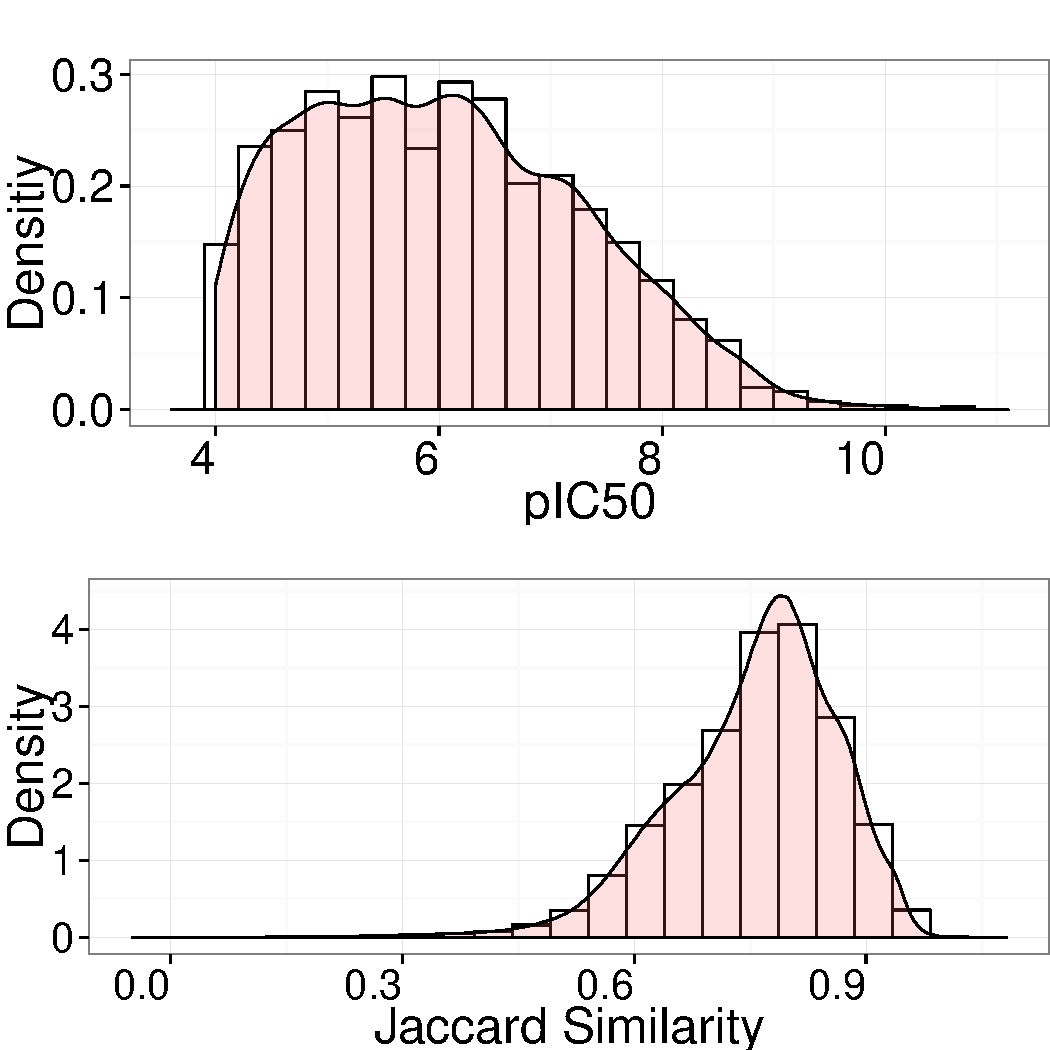
\includegraphics[width=\maxwidth]{figure/unnamed-chunk-25} 

}

\caption[Density of the response variable (upper panel)]{Density of the response variable (upper panel). Pairwise Compound Jaccard Similarity (bottom pannel)\label{fig:unnamed-chunk-25}}
\end{figure}


\end{knitrout}


%\newpage
Before any modeling attempt, it is interesting to know which is the maximum performance achievable {\it on the basis} of the uncertainty of the available data.\cite{cortesGP}
To this aim, we consider the experimental uncertainty and the size of our dataset. 
In this case, a Gaussian Process (GP) model was trained in Matlab (data not shown) where the experimental uncertainty was optimized as a hyperparameter. The obtained value was 0.60 pIC50 units.
This value is in accordance with the recently published value of 0.68 pIC50 units for public IC50 data.\cite{kramerIC50}
With the function 'MaxPerf', we can calculate the maximum achievable performance:

\begin{knitrout}
\definecolor{shadecolor}{rgb}{0.969, 0.969, 0.969}\color{fgcolor}\begin{kframe}
\begin{alltt}
\hlstd{max_performance} \hlkwb{<-} \hlkwd{MaxPerf}\hlstd{(}\hlkwc{meanNoise}\hlstd{=}\hlnum{0}\hlstd{,}\hlkwc{sdNoise}\hlstd{=}\hlnum{0.6}\hlstd{,}
                           \hlkwc{meanResp}\hlstd{=}\hlkwd{mean}\hlstd{(bioactivity),}
                           \hlkwc{sdResp}\hlstd{=}\hlkwd{sd}\hlstd{(bioactivity),}
                           \hlkwc{lenPred}\hlstd{=}\hlnum{800}\hlstd{,}\hlkwc{tmar} \hlstd{=} \hlnum{0.2}\hlstd{,}
                           \hlkwc{bmar} \hlstd{=} \hlnum{0.2}\hlstd{,} \hlkwc{rmar} \hlstd{=} \hlnum{0.2}\hlstd{,}
                           \hlkwc{lmar} \hlstd{=} \hlnum{0.2}\hlstd{)}
\end{alltt}


{\ttfamily\noindent\bfseries\color{errorcolor}{\#\# Error: unused arguments (meanResp = mean(bioactivity), sdResp = sd(bioactivity))}}\begin{alltt}
\hlkwd{grid.arrange}\hlstd{(max_performance}\hlopt{$}\hlstd{p1,max_performance}\hlopt{$}\hlstd{p2,}
             \hlstd{max_performance}\hlopt{$}\hlstd{p3,max_performance}\hlopt{$}\hlstd{p4,}\hlkwc{nrow}\hlstd{=}\hlnum{2}\hlstd{)}
\end{alltt}


{\ttfamily\noindent\bfseries\color{errorcolor}{\#\# Error: object 'max\_performance' not found}}\end{kframe}
\end{knitrout}

The function returns a list of four plots, to which further layers can be added given that they are {\it ggplot} objects.
Some graphical arguments are already available in the function "MaxPerf".
In the example given above, the margin of the plots is controlled with the arguments "tmar", "bmar", "rmar", and "lmar",
which respectively correspond to the top, bottom, right and left margins.
As we can see from Figure 3, the maxima achievable values for the correlation metrics are far from one.
Hence the importance of assessing the theoretical maximum performance the models can avhieve on the basis of the uncertainty of the experimental measurements.
\section{Statistical Pre-processing}
Bioactivity annotations in ChEMBL are sometimes redundant, 
meaning that for a given target-compound combination there are more than one annotated values.
To avoid this issue, we will remove redundant pairs and will keep the mean bioactivity value for those repeated compound-target combinations.
Further information in this respect will appear in a future publication.
In order to remove duplicate values, we run the file \verb|"remove_duplicates.R":|
\begin{knitrout}
\definecolor{shadecolor}{rgb}{0.969, 0.969, 0.969}\color{fgcolor}\begin{kframe}
\begin{alltt}
\hlkwd{source}\hlstd{(}\hlstr{"remove_duplicates.R"}\hlstd{)}
\end{alltt}
\end{kframe}
\end{knitrout}

The dataset without repeated repetitions will be saved to the file \verb|"Whole_dataset.rds".|
The dataset with only (i) compound descriptors, PaDEL and Morgan fingerprints, and (ii) amino acid descriptors
will be saved to the files \verb|"Whole_dataset_compound_descriptors.rds"| and \verb|"Whole_dataset_aa_descriptors.rds"|
respectively. All variables created while running the file \verb|"remove_duplicates.R"| will be saved to the file\\
\verb|"data_processing_repetitions_COX.RData"|.

In cases where no repeated bioactivities are present for the same datapoint, 
the different descriptors blocks (PaDEL, Morgan fingerprints and amino acid descriptors in this case)
can be simply stacked horizontally with the function "cbind".

Subsequently, we load the dataset without repetitions generated in the previous step. 
In addition, we remove those columns not containing descriptors (e.g. compound names):
\begin{knitrout}
\definecolor{shadecolor}{rgb}{0.969, 0.969, 0.969}\color{fgcolor}\begin{kframe}
\begin{alltt}
\hlstd{dataset} \hlkwb{<-} \hlkwd{readRDS}\hlstd{(}\hlstr{"Whole_dataset.rds"}\hlstd{)}
\hlstd{killset} \hlkwb{<-} \hlkwd{expression}\hlstd{(}\hlkwd{c}\hlstd{(tid, pref_name, accession,}
    \hlstd{organism, chembl_id, standard_value, standard_units,}
    \hlstd{standard_type, chembl_id.1, Name, Name.1, Name.2,}
    \hlstd{rows))}
\hlstd{bioactivity} \hlkwb{<-} \hlstd{dataset}\hlopt{$}\hlstd{standard_value}
\hlstd{compound_IDs} \hlkwb{<-} \hlstd{dataset}\hlopt{$}\hlstd{chembl_id.1}
\hlstd{dataset} \hlkwb{<-} \hlkwd{subset}\hlstd{(dataset,} \hlkwc{select} \hlstd{=} \hlopt{-}\hlkwd{eval}\hlstd{(killset))}
\end{alltt}
\end{kframe}
\end{knitrout}


Subsequently, we split the dataset into training (70\%) and hold-out (external; 30\%) sets that will be used to assess the predictive ability of the models. Furthermore, we remove the following descriptors: (i) those with a variance close to zero (near-zero variance), and (ii) those highly correlated:
\begin{knitrout}
\definecolor{shadecolor}{rgb}{0.969, 0.969, 0.969}\color{fgcolor}\begin{kframe}
\begin{alltt}
\hlcom{# Split the dataset into a training and holdout set}
\hlstd{dataset} \hlkwb{<-} \hlkwd{SplitSet}\hlstd{(compound_IDs, dataset, bioactivity,}
    \hlkwc{percentage} \hlstd{=} \hlnum{30}\hlstd{,} \hlkwc{seed} \hlstd{=} \hlnum{1}\hlstd{)}

\hlcom{# Remove the descriptors that are highly correlated}
\hlcom{# or have low variance}
\hlstd{dataset} \hlkwb{<-} \hlkwd{RemoveNearZeroVarianceFeatures}\hlstd{(dataset,}
    \hlkwc{frequencyCutoff} \hlstd{=} \hlnum{30}\hlopt{/}\hlnum{1}\hlstd{)}
\hlstd{dataset} \hlkwb{<-} \hlkwd{RemoveHighlyCorrelatedFeatures}\hlstd{(dataset)}
\end{alltt}
\end{kframe}
\end{knitrout}


We convert the descriptors to z-scores by centering them to zero mean and scaling their values to unit variance:
\begin{knitrout}
\definecolor{shadecolor}{rgb}{0.969, 0.969, 0.969}\color{fgcolor}\begin{kframe}
\begin{alltt}
\hlstd{dataset} \hlkwb{<-} \hlkwd{PreProcess}\hlstd{(dataset)}
\end{alltt}
\end{kframe}
\end{knitrout}


Given that cross-validation (CV) will be used to optimize the hyperparameters of the models, we divide the training set in 5 folds:
\begin{knitrout}
\definecolor{shadecolor}{rgb}{0.969, 0.969, 0.969}\color{fgcolor}\begin{kframe}
\begin{alltt}
\hlstd{dataset} \hlkwb{<-} \hlkwd{GetCVTrainControl}\hlstd{(dataset,} \hlkwc{seed} \hlstd{=} \hlnum{1}\hlstd{,} \hlkwc{folds} \hlstd{=} \hlnum{5}\hlstd{,}
    \hlkwc{repeats} \hlstd{=} \hlnum{1}\hlstd{,} \hlkwc{returnResamp} \hlstd{=} \hlstr{"none"}\hlstd{,} \hlkwc{returnData} \hlstd{=} \hlnum{FALSE}\hlstd{,}
    \hlkwc{savePredictions} \hlstd{=} \hlnum{TRUE}\hlstd{,} \hlkwc{verboseIter} \hlstd{=} \hlnum{TRUE}\hlstd{,} \hlkwc{allowParallel} \hlstd{=} \hlnum{TRUE}\hlstd{,}
    \hlkwc{index} \hlstd{=} \hlkwd{createMultiFolds}\hlstd{(y.train,} \hlkwc{k} \hlstd{= folds,} \hlkwc{times} \hlstd{= repeats))}
\hlkwd{saveRDS}\hlstd{(dataset,} \hlkwc{file} \hlstd{=} \hlstr{"dataset_COX_preprocessed.rda"}\hlstd{)}
\end{alltt}
\end{kframe}
\end{knitrout}

All models are trained with the same CV options, {\it i.e.} hte arguments of the function 'GetCVTrainControl' to allow ensemble modeling (see below).
It is important to mention that the functions presented in the previous code blocks depend on functions from the {\it caret} package, namely: 
\begin{itemize}
\item RemoveNearZeroVarianceFeatures : nearZeroVar
\item RemoveHighlyCorrelatedFeatures : findCorrelation
\item PreProcess : preProcess
\item GetCVTrainControl : trainControl
\end{itemize}
Experienced users might want to control more arguments of the underlying {\it caret} functions.
This is certainly possible as the arguments given to the {\it camb} functions will be subsequently given to the {\it caret} counterparts.
The default values of these function however permit the less experienced user to fo throught the statistical preprocessing
steps with ease, though guaranteeing that the choice of the argument values is reasonable.


\section{Model Training}
In the following section we will present the different steps required to train a PCM model with {\it camb}.
\begin{knitrout}
\definecolor{shadecolor}{rgb}{0.969, 0.969, 0.969}\color{fgcolor}\begin{kframe}
\begin{alltt}
\hlstd{dataset} \hlkwb{<-} \hlkwd{readRDS}\hlstd{(}\hlstr{"dataset_COX_preprocessed.rda"}\hlstd{)}
\hlcom{# Number of cores to be used during model training}
\hlstd{cores} \hlkwb{<-} \hlnum{3}
\hlkwd{registerDoMC}\hlstd{(cores)}
\end{alltt}
\end{kframe}
\end{knitrout}


\subsection{Support Vector Machines (SVM)}
Firstly, a SVM will be trained \cite{svmreview}.
We define an exponential grid (base 2) to optimize the hyperparameters:

\begin{knitrout}
\definecolor{shadecolor}{rgb}{0.969, 0.969, 0.969}\color{fgcolor}\begin{kframe}
\begin{alltt}
\hlstd{method} \hlkwb{<-} \hlstr{"svmRadial"}
\hlstd{exp_grid} \hlkwb{<-} \hlkwd{expGrid}\hlstd{(}\hlkwc{power.from} \hlstd{=} \hlopt{-}\hlnum{8}\hlstd{,} \hlkwc{power.to} \hlstd{=} \hlopt{-}\hlnum{6}\hlstd{,}
    \hlkwc{power.by} \hlstd{=} \hlnum{2}\hlstd{,} \hlkwc{base} \hlstd{=} \hlnum{2}\hlstd{)}
\hlstd{tune.grid} \hlkwb{<-} \hlkwd{expand.grid}\hlstd{(}\hlkwc{.sigma} \hlstd{= exp_grid)}
\end{alltt}
\end{kframe}
\end{knitrout}


Training (based on the {\it caret} function "train":
\begin{knitrout}
\definecolor{shadecolor}{rgb}{0.969, 0.969, 0.969}\color{fgcolor}\begin{kframe}
\begin{alltt}
\hlstd{modelCoxSVMrad} \hlkwb{<-} \hlkwd{train}\hlstd{(dataset}\hlopt{$}\hlstd{x.train, dataset}\hlopt{$}\hlstd{y.train,}
    \hlstd{method,} \hlkwc{tuneGrid} \hlstd{= tune.grid,} \hlkwc{trControl} \hlstd{= dataset}\hlopt{$}\hlstd{trControl)}
\hlkwd{saveRDS}\hlstd{(modelCoxSVMrad,} \hlkwc{file} \hlstd{=} \hlstr{"model_SVM.rds"}\hlstd{)}
\end{alltt}
\end{kframe}
\end{knitrout}


\subsection{Random Forest}
We proceed similarly in the case of a random forest (RF) model\cite{rf}.

\begin{knitrout}
\definecolor{shadecolor}{rgb}{0.969, 0.969, 0.969}\color{fgcolor}\begin{kframe}
\begin{alltt}
\hlstd{method} \hlkwb{<-} \hlstr{"rf"}
\hlstd{modelCoxRF} \hlkwb{<-} \hlkwd{train}\hlstd{(dataset}\hlopt{$}\hlstd{x.train, dataset}\hlopt{$}\hlstd{y.train,}
    \hlstd{method,} \hlkwc{trControl} \hlstd{= dataset}\hlopt{$}\hlstd{trControl)}
\hlkwd{saveRDS}\hlstd{(modelCoxRF,} \hlkwc{file} \hlstd{=} \hlstr{"model_RF.rds"}\hlstd{)}
\end{alltt}
\end{kframe}
\end{knitrout}

%Loading the RF model.



\subsection{Gradient Boosting Machine}
We proceed similarly in the case of a gradient boosting machine (GBM) model\cite{gbm}.

\begin{knitrout}
\definecolor{shadecolor}{rgb}{0.969, 0.969, 0.969}\color{fgcolor}\begin{kframe}
\begin{alltt}
\hlstd{method} \hlkwb{<-} \hlstr{"gbm"}
\hlstd{tune.grid} \hlkwb{<-} \hlkwd{expand.grid}\hlstd{(}\hlkwc{.shrinkage} \hlstd{=} \hlkwd{c}\hlstd{(}\hlnum{0.04}\hlstd{,} \hlnum{0.08}\hlstd{,}
    \hlnum{0.12}\hlstd{,} \hlnum{0.16}\hlstd{),} \hlkwc{.n.trees} \hlstd{=} \hlkwd{c}\hlstd{(}\hlnum{500}\hlstd{),} \hlkwc{.interaction.depth} \hlstd{=} \hlkwd{c}\hlstd{(}\hlnum{25}\hlstd{))}
\hlstd{modelCoxGBM} \hlkwb{<-} \hlkwd{train}\hlstd{(dataset}\hlopt{$}\hlstd{x.train, dataset}\hlopt{$}\hlstd{y.train,}
    \hlstd{method,} \hlkwc{tuneGrid} \hlstd{= tune.grid,} \hlkwc{trControl} \hlstd{= dataset}\hlopt{$}\hlstd{trControl)}
\hlkwd{saveRDS}\hlstd{(modelCoxGBM,} \hlkwc{file} \hlstd{=} \hlstr{"model_GBM.rds"}\hlstd{)}
\end{alltt}
\end{kframe}
\end{knitrout}



\section{Model Evaluation}

Once the models are trained, the cross validated metrics can be calculated:
We assume that the metric used for the choice of the best combination of hyperparameters is 'RMSE',
which is normally considered as the aim of bioactivity modeling, {\it i.e.} how far (on average) are our 
predictions from the real the bioactivity values?.
In the following we focus on the RF model, though the same steps can be applied to the GBM and SVM models.

\begin{knitrout}
\definecolor{shadecolor}{rgb}{0.969, 0.969, 0.969}\color{fgcolor}\begin{kframe}
\begin{alltt}
\hlstd{RMSE_CV_rf} \hlkwb{=} \hlkwd{RMSE_CV}\hlstd{(modelCoxRF,} \hlkwc{digits} \hlstd{=} \hlnum{3}\hlstd{)}
\hlstd{Rsquared_CV_rf} \hlkwb{=} \hlkwd{Rsquared_CV}\hlstd{(modelCoxRF,} \hlkwc{digits} \hlstd{=} \hlnum{3}\hlstd{)}
\hlkwd{print}\hlstd{(RMSE_CV_rf)}
\end{alltt}
\begin{verbatim}
## [1] 0.775
\end{verbatim}
\begin{alltt}
\hlkwd{print}\hlstd{(Rsquared_CV_rf)}
\end{alltt}
\begin{verbatim}
## [1] 0.5914
\end{verbatim}
\end{kframe}
\end{knitrout}


On the basis of the soundness of the obtained models, assessed through the value of the cross-validated metrics, 
we proceed to predict the values for the external (hold-out) set:
\begin{knitrout}
\definecolor{shadecolor}{rgb}{0.969, 0.969, 0.969}\color{fgcolor}\begin{kframe}
\begin{alltt}
\hlstd{holdout.predictions} \hlkwb{<-} \hlkwd{as.vector}\hlstd{(}\hlkwd{predict}\hlstd{(modelCoxRF}\hlopt{$}\hlstd{finalModel,}
    \hlkwc{newdata} \hlstd{= dataset}\hlopt{$}\hlstd{x.holdout))}
\end{alltt}
\end{kframe}
\end{knitrout}


The predictive ability of the models is evaluated by calculation the following statistical metrics:

{\bf Internal validation:}

\begin{equation}
q_{{\it int}}^{2} \ or \  R_{tr}^{2}  = 1 - \frac {\sum_{i=1}^{N_{tr}} (y_{i} - \widetilde{y}_{i})^{2}} {\sum_{i=1}^{N_{int}} (y_{i} - \bar{y}_{tr})^{2}}
\end{equation}
% cross-validated correlation coefficient

\begin{equation}
RMSE_{int} = \frac {\sqrt {(y_i - \widetilde{y}_i)^{2}}} {N}
\end{equation}

where $N$, $y_i$, $\widetilde{y}_i$ and $\bar{y}_{tr}$ represent the size of the training set, the observed, the predicted and the averaged values of the response variable for those datapoints included in the training set. The {\it i}th position within the training set is defined by {\it i}.\\  


{\bf External validation:}


\begin{equation}
Q_{1\ {\it ext}}^{2} = 1 - \frac {\sum_{j=1}^{N_{ext}} (y_j-\widetilde{y}_j)^{2}}  {\sum_{j=1}^{N_{ext}} (y_j - \bar{y}_{tr})^{2}}
\end{equation}

\begin{equation}
Q_{2\ {\it ext}}^{2} = 1 - \frac {\sum_{j=1}^{N_{ext}} (y_j-\widetilde{y}_j)^{2}}  {\sum_{j=1}^{N_{ext}} (y_j - \bar{y}_{ext})^{2}}
\end{equation}

\begin{equation}
Q_{3\ {\it ext}}^{2} = 1 - \frac {[\sum_{j=1}^{N_{ext}} (y_j-\widetilde{y}_j)^{2}] / N_{ext} }  {[ \sum_{j=1}^{N_{tr}} (y_j - \bar{y}_{tr})^{2}] / N_{tr}}
\end{equation}

\begin{equation}
RMSE_{ext} = \frac {\sqrt {(y_i - \widetilde{y}_i)^{2}}} {N} 
\end{equation}

\begin{equation}
R_{ext}^{2} = \frac {{\sum_{i=1}^{N_{ext}} (y_{i} - \bar{y}_{ext})}  (\widetilde{y}_{i} - \overset{-}{\widetilde{y}_{ext}})} 
{\sqrt{\sum_{i=1}^{N_{ext}} (y_{i} - \bar{y}_{ext})^{2} \sum{ (\widetilde{y}_{i} - \overset{-}{\widetilde{y}_{ext}})^{2}}}}
\end{equation}

\begin{equation}
R_{0\:ext}^2 = 1 - \frac {\sum_{j=1}^{N_{ext}} (y_{j} - \widetilde{y}_{j}^{ r0})^{2}} {\sum_{j=1}^{N_{ext}} (y_{j} - \bar{y}_{ext})^{2}} 
\end{equation}

where $N$, $y_j$, $\widetilde{y}_j$, and $\bar{y}_{ext}$ represent the size of the training set, the observed, the predicted, and the averaged values of the response variable for those datapoints comprising the external set.  $R_{0\:ext}^2$ is the square of the coefficient of determination through the origin, being $\widetilde{y}_{j}^{ r0} = k \widetilde{y}_j$ the regression through the origin (observed versus predicted) and $k$ its slope.\\
For a detailed discussion of both the evaluation of the predictive ability through the external set and about the three different formulations for $Q^{2}_{ext}$, namely $Q_{1\ {\it ext}}^{2}$, $Q_{2\ {\it ext}}^{2}$, and $Q_{3\ {\it ext}}^{2}$, see ref.\cite{consonni}. 
To be considered as predictive, a model must satisfy the following criteria:\cite{beware,earnest}
\\
\begin{enumerate}
\item $q_{{\it int}}^{2} > 0.5$
\item $R_{ext}^2 > 0.6$
\item $ \frac {(R_{ext}^2 - R_{0\:ext}^2)} {R_{ext}^2} < 0.1$
\item $0.85 \leq k \leq 1.15$
\end{enumerate}

The metrics for the external validation are given by:
\begin{knitrout}
\definecolor{shadecolor}{rgb}{0.969, 0.969, 0.969}\color{fgcolor}\begin{kframe}
\begin{alltt}
\hlstd{MetricsRf} \hlkwb{<-} \hlkwd{Validation}\hlstd{(predholdout.predictions, dataset}\hlopt{$}\hlstd{y.holdout,}
    \hlkwc{resp_tr} \hlstd{= bioactivities)}
\end{alltt}
\end{kframe}
\end{knitrout}

The argument \verb|"resp_tr"|, requires the bioactivity values of the datapoints present in the training set.
These values are required by the metrics $Q_{1}$ and $Q_{3}$ (see above).

To visualize the correlation between predicted and observed values, we can use the 'CorrelationPlot' function:




\begin{knitrout}
\definecolor{shadecolor}{rgb}{0.969, 0.969, 0.969}\color{fgcolor}\begin{kframe}
\begin{alltt}
\hlkwd{CorrelationPlot}\hlstd{(}\hlkwc{pred} \hlstd{= holdout.predictions,} \hlkwc{obs} \hlstd{= dataset}\hlopt{$}\hlstd{y.holdout,}
    \hlkwc{PointSize} \hlstd{=} \hlnum{3}\hlstd{,} \hlkwc{ColMargin} \hlstd{=} \hlstr{"blue"}\hlstd{,} \hlkwc{TitleSize} \hlstd{=} \hlnum{26}\hlstd{,}
    \hlkwc{XAxisSize} \hlstd{=} \hlnum{20}\hlstd{,} \hlkwc{YAxisSize} \hlstd{=} \hlnum{20}\hlstd{,} \hlkwc{TitleAxesSize} \hlstd{=} \hlnum{24}\hlstd{,}
    \hlkwc{margin} \hlstd{=} \hlnum{2}\hlstd{,} \hlkwc{PointColor} \hlstd{=} \hlstr{"black"}\hlstd{,} \hlkwc{PointShape} \hlstd{=} \hlnum{16}\hlstd{,}
    \hlkwc{MarginWidth} \hlstd{=} \hlnum{1}\hlstd{,} \hlkwc{AngleLab} \hlstd{=} \hlnum{0}\hlstd{,} \hlkwc{xlab} \hlstd{=} \hlstr{"Observed"}\hlstd{,}
    \hlkwc{ylab} \hlstd{=} \hlstr{"Predicted"}\hlstd{)}
\end{alltt}


{\ttfamily\noindent\bfseries\color{errorcolor}{\#\# Error: could not find function "{}CorrelationPlot"{}}}\end{kframe}
\end{knitrout}


\section{Ensemble Modeling}
In the following section, two ensemble modeling techniques will be applied, namely greedy optimization and model stacking.
Further information can be found in ref \cite{caretEnsemble} and \cite{caruana}.



To get (i) the training set, (ii) the external set, (iii) the transformation applied to center and scale the descriptors before model training, and (iv) the model training options, we run the following lines of code:
\begin{knitrout}
\definecolor{shadecolor}{rgb}{0.969, 0.969, 0.969}\color{fgcolor}\begin{kframe}
\begin{alltt}
\hlstd{data} \hlkwb{<-} \hlkwd{list}\hlstd{()}
\hlkwd{attach}\hlstd{(dataset)}
\hlstd{data}\hlopt{$}\hlstd{transformation} \hlkwb{<-} \hlstd{transformation}
\hlstd{data}\hlopt{$}\hlstd{x.train} \hlkwb{<-} \hlstd{x.train}
\hlstd{data}\hlopt{$}\hlstd{y.train} \hlkwb{<-} \hlstd{y.train}
\hlstd{data}\hlopt{$}\hlstd{x.test} \hlkwb{<-} \hlstd{x.holdout}  \hlcom{# external set}
\hlstd{data}\hlopt{$}\hlstd{y.test} \hlkwb{<-} \hlstd{y.holdout}  \hlcom{# external set}
\hlstd{data}\hlopt{$}\hlstd{trControl} \hlkwb{<-} \hlstd{trControl}
\hlkwd{saveRDS}\hlstd{(data,} \hlkwc{file} \hlstd{=} \hlstr{"data_ensemble.rds"}\hlstd{)}
\hlkwd{detach}\hlstd{(dataset)}
\end{alltt}
\end{kframe}
\end{knitrout}

Subsequently, we load the models previously trained.
The list of models is in the file modelsEnsemble.
Once all models have been loaded, we create the following ensemble:
\begin{knitrout}
\definecolor{shadecolor}{rgb}{0.969, 0.969, 0.969}\color{fgcolor}\begin{kframe}
\begin{alltt}
\hlstd{greedy} \hlkwb{<-} \hlkwd{caretEnsemble}\hlstd{(all.models,} \hlkwc{iter} \hlstd{=} \hlnum{1000L}\hlstd{)}
\hlkwd{sort}\hlstd{(greedy}\hlopt{$}\hlstd{weights,} \hlkwc{decreasing} \hlstd{=} \hlnum{TRUE}\hlstd{)}

\hlstd{all.models} \hlkwb{<-} \hlkwd{list}\hlstd{()}
\hlstd{models} \hlkwb{<-} \hlkwd{as.vector}\hlstd{(}\hlkwd{read.table}\hlstd{(}\hlstr{"modelsEnsemble"}\hlstd{)}\hlopt{$}\hlstd{V1)}

\hlkwa{for} \hlstd{(i} \hlkwa{in} \hlnum{1}\hlopt{:}\hlkwd{length}\hlstd{(models)) \{}
    \hlstd{model_load} \hlkwb{=} \hlkwd{paste}\hlstd{(}\hlstr{"readRDS('"}\hlstd{, models[i],} \hlstr{"')"}\hlstd{,}
        \hlkwc{sep} \hlstd{=} \hlstr{""}\hlstd{)}
    \hlkwd{assign}\hlstd{(}\hlkwd{paste}\hlstd{(}\hlstr{"model_"}\hlstd{, i,} \hlkwc{sep} \hlstd{=} \hlstr{""}\hlstd{),} \hlkwd{eval}\hlstd{(}\hlkwd{parse}\hlstd{(}\hlkwc{text} \hlstd{= model_load)))}
    \hlstd{all.models[[}\hlkwd{length}\hlstd{(all.models)} \hlopt{+} \hlnum{1}\hlstd{]]} \hlkwb{<-} \hlkwd{eval}\hlstd{(}\hlkwd{parse}\hlstd{(}\hlkwc{text} \hlstd{=} \hlkwd{paste}\hlstd{(}\hlstr{"model_"}\hlstd{,}
        \hlstd{i,} \hlkwc{sep} \hlstd{=} \hlstr{""}\hlstd{)))}
\hlstd{\}}

\hlkwd{names}\hlstd{(all.models)} \hlkwb{<-} \hlkwd{sapply}\hlstd{(all.models,} \hlkwa{function}\hlstd{(}\hlkwc{x}\hlstd{) x}\hlopt{$}\hlstd{method)}
\hlkwd{sort}\hlstd{(}\hlkwd{sapply}\hlstd{(all.models,} \hlkwa{function}\hlstd{(}\hlkwc{x}\hlstd{)} \hlkwd{min}\hlstd{(}\hlkwd{as.vector}\hlstd{(}\hlkwd{na.omit}\hlstd{(x}\hlopt{$}\hlstd{results}\hlopt{$}\hlstd{RMSE)))))}
\end{alltt}
\end{kframe}
\end{knitrout}


Once all models have been loaded, we create the following ensemble:
  %\begin{enumerate}
%\item Greedy (now it can only optimize the hold-out RMSE)
\begin{knitrout}
\definecolor{shadecolor}{rgb}{0.969, 0.969, 0.969}\color{fgcolor}\begin{kframe}
\begin{alltt}
\hlstd{greedy} \hlkwb{<-} \hlkwd{caretEnsemble}\hlstd{(all.models,} \hlkwc{iter} \hlstd{=} \hlnum{1000L}\hlstd{)}
\hlkwd{sort}\hlstd{(greedy}\hlopt{$}\hlstd{weights,} \hlkwc{decreasing} \hlstd{=} \hlnum{TRUE}\hlstd{)}
\end{alltt}
\end{kframe}
\end{knitrout}


%\item Model Stacking
\begin{knitrout}
\definecolor{shadecolor}{rgb}{0.969, 0.969, 0.969}\color{fgcolor}\begin{kframe}
\begin{alltt}
\hlcom{  # make a linear regression ensemble}
  linear <- \hlkwd{caretStack}(all.models, method=\hlstr{'glm'})
\hlkwd{summary}(linear$ens_model$finalModel)

\hlcom{# make Elastic Net ensemble}
enet_ens <- \hlkwd{caretStack}(all.models, method=\hlstr{'enet'})
coefs_enet_ens <- enet_ens$ens_model$finalModel$beta.pure +
[\hlkwd{ncol}(enet_ens$ens_model$finalModel$beta.pure)+1,]

\hlcom{# make SVM linear ensemble}
trControl <- \hlkwd{trainControl}(method = \hlstr{"cv"},  number=5)
tune.grid <- \hlkwd{expand.grid}(.C=\hlkwd{expGrid}(power.from=-14,
                                    power.to=10,power.by=1,base=2))
linear_svm <- \hlkwd{caretStack}(all.models, method=\hlstr{'svmLinear'},
                         trControl=trControl,tuneGrid=tune.grid)

\hlcom{# make SVM radial ensemble}
trControl <- \hlkwd{trainControl}(method = \hlstr{"cv"},  number=5)
tune.grid <- \hlkwd{expand.grid}(.sigma=\hlkwd{expGrid}(power.from=-14,
                                        power.to=10,power.by=1,base=2),
                         .C=\hlkwd{expGrid}(power.from=-14,power.to=10,
                                    power.by=2,base=2))
radial_svm <- \hlkwd{caretStack}(all.models, method=\hlstr{'svmRadial'},
                         trControl=trControl,tuneGrid=tune.grid)
\end{alltt}
\end{kframe}
\end{knitrout}

%\end{enumerate}
We proceed to predict the bioactivities for the external (hold-out) set,
\begin{knitrout}
\definecolor{shadecolor}{rgb}{0.969, 0.969, 0.969}\color{fgcolor}\begin{kframe}
\begin{alltt}
preds <- \hlkwd{data.frame}(\hlkwd{sapply}(all.models, predict, newdata=dataa$x.test))
preds$ENS_greedy <- \hlkwd{predict}(greedy, newdata=dataa$x.test)
preds$ENS_linear <- \hlkwd{predict}(linear, newdata=dataa$x.test)
preds$ENS_enet <- \hlkwd{predict}(enet_ens, newdata=x.test)
preds$ENS_SVMrad <- \hlkwd{predict}(radial_svm, newdata=x.test)c
preds$ENS_SVMlin <- \hlkwd{predict}(linear_svm, newdata=x.test)
\end{alltt}
\end{kframe}
\end{knitrout}


and we calculate the values of the statistical metrics:
  
\begin{knitrout}
\definecolor{shadecolor}{rgb}{0.969, 0.969, 0.969}\color{fgcolor}\begin{kframe}
\begin{alltt}
\hlcom{# Calculate metrics (We could also have applied}
\hlcom{# Validation instead.)}
\hlstd{Q2_1s} \hlkwb{<-} \hlkwd{apply}\hlstd{(preds,} \hlnum{2}\hlstd{,} \hlkwa{function}\hlstd{(}\hlkwc{x}\hlstd{)} \hlkwd{Qsquared1}\hlstd{(x, dataa}\hlopt{$}\hlstd{y.test))}
\hlstd{Q2_2s} \hlkwb{<-} \hlkwd{apply}\hlstd{(preds,} \hlnum{2}\hlstd{,} \hlkwa{function}\hlstd{(}\hlkwc{x}\hlstd{)} \hlkwd{Qsquared2}\hlstd{(x, dataa}\hlopt{$}\hlstd{y.test))}
\hlstd{Q2_3s} \hlkwb{<-} \hlkwd{apply}\hlstd{(preds,} \hlnum{2}\hlstd{,} \hlkwa{function}\hlstd{(}\hlkwc{x}\hlstd{)} \hlkwd{Qsquared3}\hlstd{(x, dataa}\hlopt{$}\hlstd{y.test))}
\hlstd{R2s} \hlkwb{<-} \hlkwd{apply}\hlstd{(preds,} \hlnum{2}\hlstd{,} \hlkwa{function}\hlstd{(}\hlkwc{x}\hlstd{)} \hlkwd{Rsquared}\hlstd{(x, dataa}\hlopt{$}\hlstd{y.test))}
\hlstd{R20s} \hlkwb{<-} \hlkwd{apply}\hlstd{(preds,} \hlnum{2}\hlstd{,} \hlkwa{function}\hlstd{(}\hlkwc{x}\hlstd{)} \hlkwd{Rsquared0}\hlstd{(x, dataa}\hlopt{$}\hlstd{y.test))}
\hlstd{RMSEs} \hlkwb{<-} \hlkwd{apply}\hlstd{(preds,} \hlnum{2}\hlstd{,} \hlkwa{function}\hlstd{(}\hlkwc{x}\hlstd{)} \hlkwd{RMSE}\hlstd{(x, dataa}\hlopt{$}\hlstd{y.test))}
\end{alltt}
\end{kframe}
\end{knitrout}

%\section{Bibliography}
\newpage
\printbibliography

\end{document}
